\begin{minipage}[c]{.45\linewidth} 
\Large \textbf{\textsf{NOM1 Prenom1}} 
 
 \normalsize Note harmonisée 12.66/20 
 
Rang 2
 
Moyenne classe harmonisée 6.92/20 
 
Commentaires : 
c1 
\end{minipage}\hfill 
\begin{minipage}[c]{.45\linewidth}  
\begin{center}
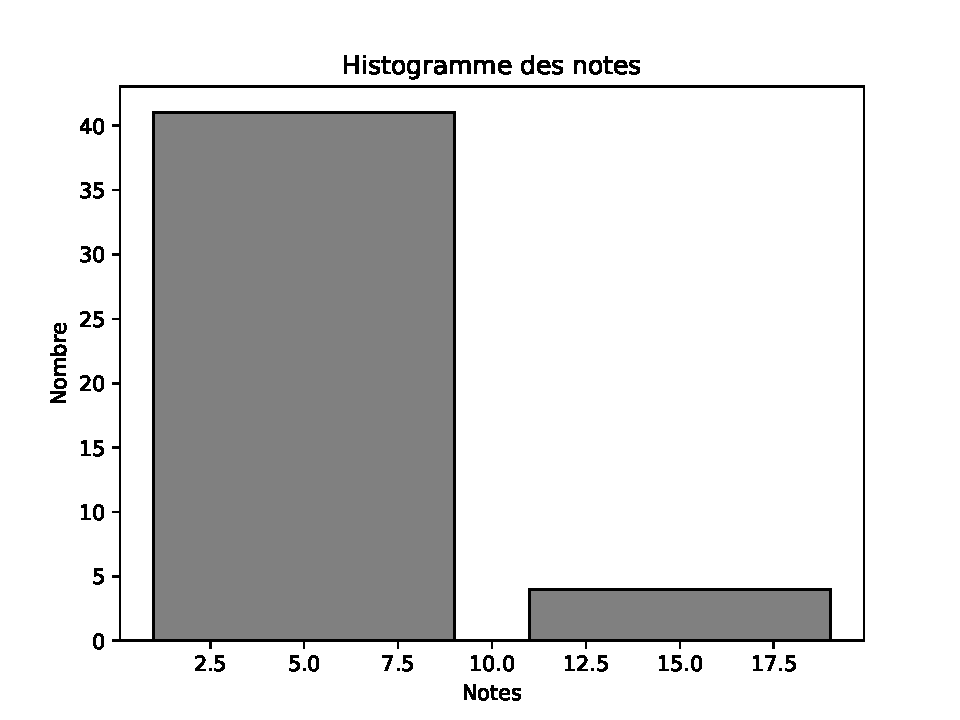
\includegraphics[width=.8\linewidth]{../histo.pdf} 
\end{center}
\end{minipage}
\footnotesize 
\begin{center} 
\begin{tabular}{|c|c|m{1cm}|c||c|c|m{1cm}|c||c|c|m{1cm}|c||c|c|m{1cm}|c|} 
\hline \textbf{Qu} & \textbf{Coef} & \textbf{Comp} & \textbf{/5} & \textbf{Qu} & \textbf{Coef} & \textbf{Comp} & \textbf{/5} & \textbf{Qu} & \textbf{Coef} & \textbf{Comp} & \textbf{/5} & \textbf{Qu} & \textbf{Coef} & \textbf{Comp} & \textbf{/5} \\ 
\hline 
\hline 
1 & 4.0 & A, A, A, C & 2.0 & 10 & 5.0 & A, A, E & 1.5 & 19 & 11.0 & A, A, A, E & 1.0 & 28 & 1.0 & M & 5.0 \\ \hline 
2 & 5.0 & A, A, C & 3.0 & 11 & 14.0 & A, A, A, A, E & 0.0 & 20 & 3.0 & A, A, E & 5.0 & 29 & 2.0 & M & 5.0 \\ \hline 
3 & 8.0 & A, A, C & 5.0 & 12 & 3.0 & A, A, E & 0.0 & 21 & 6.0 & A, A, E & 5.0 & 30 & 2.0 & A, M & 5.0 \\ \hline 
4 & 3.0 & A, A, C & 2.0 & 13 & 7.0 & A, A, A, E & 0.0 & 22 & 9.0 & A, A, E & 5.0 & 31 & 3.0 & C, M & 5.0 \\ \hline 
5 & 6.0 & A, A, E & 4.2 & 14 & 11.0 & A, A, A, E & 0.0 & 23 & 6.0 & A, A, E & 4.0 & 32 & 2.0 & C, M & 5.0 \\ \hline 
6 & 9.0 & A, A, E & 4.0 & 15 & 5.0 & C, E & 3.5 & 24 & 10.0 & A, A, A, E & 1.0 & 33 & 3.0 & C, M & 5.0 \\ \hline 
7 & 2.0 & E & 4.0 & 16 & 2.0 & C, E & 5.0 & 25 & 4.0 & A, A, M & 5.0 &  &  &  &  \\ \hline 

8 & 1.0 & E & 1.0 & 17 & 5.0 & A, A, C, E & 1.0 & 26 & 5.0 & A, A, M & 5.0 &  &  &  &  \\ \hline 

9 & 4.0 & A, A, E & 5.0 & 18 & 6.0 & A, A, C, E & 5.0 & 27 & 6.0 & A, M & 5.0 &  &  &  &  \\ \hline 

\end{tabular} 
\end{center} 
\normalsize 
 
\footnotesize 
\begin{center} 
\begin{tabular}{|p{.7\linewidth}|c|} 
\hline 
Compétences  & Taux \\ \hline \hline 
An1.C1 -- CdC (req, uc)&60.0 \%(=)\\ \hline 
An1.C2 -- Impact environnemental&22.0 \% ($\searrow$ 60\,\%)\\ \hline 
An2.C3 -- Frontière de l’étude&80.0 \% ($\nearrow$ 22\,\%)\\ \hline 
An2.C4 -- Milieu extérieur&40.0 \% ($\searrow$ 80\,\%)\\ \hline 
An2.C5 -- Flux échangés&54.0 \% ($\nearrow$ 40\,\%)\\ \hline 
An3.C1 -- Architectures fonctionnelle et structurelle&80.0 \% ($\nearrow$ 54\,\%)\\ \hline 
An3.C2 -- Diagrammes de définition de blocs&100.0 \% ($\nearrow$ 80\,\%)\\ \hline 
An3.C3 -- Chaîne directe&83.0 \% ($\searrow$ 100\,\%)\\ \hline 
An3.C4 -- Dystème asservi&100.0 \% ($\nearrow$ 83\,\%)\\ \hline 
An3.C6 -- Chaîne d’information et d'énergie&17.0 \% ($\searrow$ 100\,\%)\\ \hline 
An3.C8 -- Diagramme paramétrique&60.0 \% ($\nearrow$ 17\,\%)\\ \hline 
An3.C9 -- Systèmes à événements discrets&25.0 \% ($\searrow$ 60\,\%)\\ \hline 
An3.C10 -- Diagramme de séquences&75.0 \% ($\nearrow$ 25\,\%)\\ \hline 
An3.C11 -- Diagramme d’états&0.0 \% ($\searrow$ 75\,\%)\\ \hline 
An3.C12 -- Réversibilité de la chaîne d’énergie&33.0 \% ($\nearrow$ 0\,\%)\\ \hline 
An3.C13 -- Source&80.0 \% ($\nearrow$ 33\,\%)\\ \hline 
An3.C14 -- Modulateur&100.0 \% ($\nearrow$ 80\,\%)\\ \hline 
An3.C15 -- Actionneur&80.0 \% ($\searrow$ 100\,\%)\\ \hline 
An3.C16 -- Chaîne de transmission&100.0 \% ($\nearrow$ 80\,\%)\\ \hline 
An4.C2 -- Quantification des écarts&25.0 \% ($\searrow$ 100\,\%)\\ \hline 
An4.C3 -- Interprétation des écarts obtenus&100.0 \% ($\nearrow$ 25\,\%)\\ \hline 
An5.C1 -- Grandeurs utilisées &0.0 \% ($\searrow$ 100\,\%)\\ \hline 
An5.C2 -- Ordres de grandeur&20.0 \% ($\nearrow$ 0\,\%)\\ \hline 
Com1.C1 -- Informations techniques&67.0 \% ($\nearrow$ 20\,\%)\\ \hline 
Com1.C2 -- Schémas cinématique, électrique, hydraulique et pneumatique&100.0 \% ($\nearrow$ 67\,\%)\\ \hline 
Com1.C3 -- Langage SysML&0.0 \% ($\searrow$ 100\,\%)\\ \hline 
Com2.C1 -- Outils de communication&100.0 \% ($\nearrow$ 0\,\%)\\ \hline 
Com2.C2 -- Langage technique&100.0 \%(=)\\ \hline 
Com2.C3 -- Schémas cinématique, électrique&100.0 \%(=)\\ \hline 
Con.C1 -- Architecture fonctionnelle et structurelle&100.0 \%(=)\\ \hline 
Con.C2 -- Correction d’un système asservi&50.0 \% ($\searrow$ 100\,\%)\\ \hline 
Con.C3 -- Système logique&100.0 \% ($\nearrow$ 50\,\%)\\ \hline 
Con.C4 -- Systèmes à événements discrets&100.0 \%(=)\\ \hline 
Con.C5 -- Structures algorithmiques&0.0 \% ($\searrow$ 100\,\%)\\ \hline 
Exp1.C1 -- Chaîne d’énergie&100.0 \% ($\nearrow$ 0\,\%)\\ \hline 
Exp1.C2 -- Chaîne d’information&100.0 \%(=)\\ \hline 
Exp1.C3 -- Paramètres influents&100.0 \%(=)\\ \hline 
Exp2.C1 -- Modèles de comportement d’un système&0.0 \% ($\searrow$ 100\,\%)\\ \hline 
Exp2.C2 -- Protocoles expérimentaux&100.0 \% ($\nearrow$ 0\,\%)\\ \hline 
Exp2.C3 -- Chaîne d’acquisition&0.0 \% ($\searrow$ 100\,\%)\\ \hline 
Exp2.C4 -- Filtrage&0.0 \%(=)\\ \hline 
Exp2.C5 -- Échantillonnage&0.0 \%(=)\\ \hline 
Exp2.C6 -- Quantification&0.0 \%(=)\\ \hline 
Exp3.C1 -- Règles de sécurité élémentaires&0.0 \%(=)\\ \hline 
Exp3.C2 -- Chaîne d'acquisition&50.0 \% ($\nearrow$ 0\,\%)\\ \hline 
Exp3.C3 -- Fréquence d’échantillonnage&100.0 \% ($\nearrow$ 50\,\%)\\ \hline 
Exp3.C4 -- Paramètres de configuration du système&0.0 \% ($\searrow$ 100\,\%)\\ \hline 
Exp3.C5 -- Réversibilité de la chaîne d’énergie&100.0 \% ($\nearrow$ 0\,\%)\\ \hline 
Exp3.C6 -- Source, modulateur, actionneur, chaîne de transmission&0.0 \% ($\searrow$ 100\,\%)\\ \hline 
Exp3.C7 -- Routines, procédures &100.0 \% ($\nearrow$ 0\,\%)\\ \hline 
Exp3.C8 -- Systèmes logiques à événements discrets&100.0 \%(=)\\ \hline 
Exp3.C9 -- Modèles de comportement&100.0 \%(=)\\ \hline 
Exp3.C10 -- Identification temporelle d’un modèle de comportement&100.0 \%(=)\\ \hline 
Exp3.C11 -- Identification fréquentielle d’un modèle de comportement&0.0 \% ($\searrow$ 100\,\%)\\ \hline 
Mod1.C1 -- Caractéristiques des grandeurs physiques&100.0 \% ($\nearrow$ 0\,\%)\\ \hline 
Mod1.C2 -- Flux de matière&100.0 \%(=)\\ \hline 
Mod1.C3 -- Flux d’information&100.0 \%(=)\\ \hline 
Mod1.C4 -- Énergie&100.0 \%(=)\\ \hline 
Mod1.C5 -- Puissance&100.0 \%(=)\\ \hline 
Mod1.C6 -- Rendement&100.0 \%(=)\\ \hline 
Mod2.C1 -- Chaîne d’énergie et d'information&100.0 \%(=)\\ \hline 
Mod2.C2 -- SLCI - Modélisation par équations différentielles&100.0 \%(=)\\ \hline 
Mod2.C3 -- SLCI - Calcul symbolique&100.0 \%(=)\\ \hline 
\end{tabular} 
\end{center} 
\normalsize 
 
